\subsection{Social Agents}
Agents represent a highly interdisciplinary field with influences and applications in several diverse areas such as economics, philosophy, logic, ecology, social science and computer science \cite{wooldridge:multiagent-systems}.
It's expectable that such a diverse field might have no universally accepted definition for agents \cite{wooldridge:intelligentagents}.

For the remainder of this section I'll, firstly, present a definition for what an Agent is and also see the notion of an intelligent agent.
I'll then continue on analysing what makes an agent social, thus defining Social Actions.
Finally, I'll move on into analysing some social agent's architectures.
By the end of this section it should be clear what requirements our agent must comply to in order to be called a social agent.

\subsubsection{Agents}
According to \cite{russell&norvig:aima}, an agent is "\textit{anything that can be viewed as perceiving its environment through sensors and acting upon that environment through actuators}".
Humans can be considered agents and so can computers.
We perceive our environment through our five senses (hearing, sight, touch, smell, and taste) and act upon it through our arms, hands, voice, etc. causing changes in the environment.
Computer programs perceive their environment through keystrokes, file contents, and network packets and act on the environment by displaying on the screen, writing files, and outputting music to the speakers, among many other sensors and actuators.

However there is a clear difference between a human being and a Unix daemon.
We do not usually think of Unix daemons as intelligent agents (although we might consider them agents).
As another example, even a light switch can be described as a very cooperative agent that invariably transmits electricity when we want it to do so; flicking the switch is the way we communicate our desire \cite{shoham:agentorientedprogramming}.
This example may sound absurd, but it is logical.

However, and following Shoham rationale in \cite{shoham:agentorientedprogramming}, considering the light bulb an agent, "\textit{does not buy us anything, since we essentially understand the mechanism sufficiently to have a simpler, mechanistic description of its behaviour}".
Therefore, it is important to understand what are intelligent agents and part from this general view of considering almost everything an agent.

In \cite{wooldridge:multiagent-systems}, Wooldridge identifies a list of capabilities that an intelligent agent is expected to possess.

\begin{description}
	\item[Reactivity] Intelligent agents must be able to respond in a timely fashion to changes in their environments.
	The environment may change while the agent is following a certain procedure, be it by the presence of other agents or by the characteristics of the environment.
	Blindly following that procedure without regard for environment changes is unwise as it may cause the agent to try to accomplish a goal that is no longer valid.
	\item[Proactiveness] Intelligent agents exhibit behaviours that will allow them to achieve their own goals. 
	\item[Social Ability] Intelligent agents are capable of interacting with other agents in order to achieve their goals.
\end{description}

As we can see, social ability is closely related with an intelligent agent's capabilities.

\subsubsection{What makes them Social?}
As we've seen, social ability is one of the main capabilities an agent must possess in order to be considered intelligent.
But what is Social Ability?
We can say that a social able agent performs Social Actions.

Consider a web browser: it exchanges messages with a web server through the Internet using a well-known protocol for communication, presenting web pages to the user on demand.
Can we consider a browser a social agent?

Even if we view both the browser and the web server as agents, this simple form of communication can hardly be considered social.
Going back to our example of Unix daemons, they are usually engaged in several exchanges of information with their peers and negotiate how to exchange this information, but that does not make them social.

As Castelfranchi puts it: "\textit{Agents are not 'agents' by virtue of the fact that they communicate;
they cannot be called 'social' because they communicate but the other way around: they communicate because they are social}" \cite{castelfranchi:socialactions}.

\begin{figure}
  \centering
    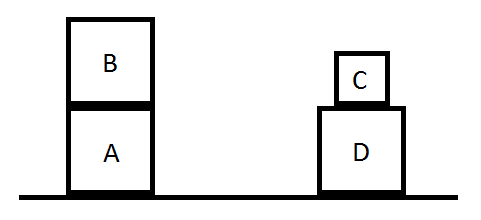
\includegraphics[width=\textwidth]{block-world-1}
  \caption{Block World initial state}
  \label{fig:block-world-1}
\end{figure}

Over the years, there as been the common misconception of considering negotiating agents as social, but as we have seen that's not always the case.
So, what makes actions social?

Imagine a block world where two agents exist, check Fig. \ref{fig:block-world-1}.
Both agents can move blocks around the world at will but cannot communicate.
The first agent, Sam, has the goal of putting both blocks A and B on the table, and the second agent, Bob, as the goal of putting block C on top of block A.
However, Bob cannot move blocks A, B, and D due to their size.
Therefore, Bob needs Sam in order to achieve its goal.

\begin{figure}
  \centering
    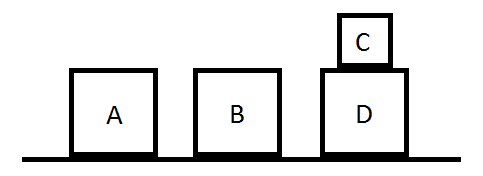
\includegraphics[width=\textwidth]{block-world-2}
  \caption{Block World after Sam's action}
  \label{fig:block-world-2}
\end{figure}

Following only its own goals, Sam will put block B on the table (check Fig. \ref{fig:block-world-2}), and Bob will then be able to put block C on top of A, completing its own goal (check Fig. \ref{fig:block-world-3}).
In this example, Sam and Bob exhibited some sort of cooperation and both achieved their own goals \footnote{This example was taken from \cite{castelfranchi:socialactions}}.

But they did so unconsciously, without knowing or having any understanding of eachother's goals, thus an action related to another agent is not necessarily social \cite{castelfranchi:individualsocialaction}.
And the opposite is also true, an action not directly related to another agent may be social in nature (consider, for example, when an agent closes a door because it doesn't want others agents looking inside the room).

\begin{figure}
  \centering
    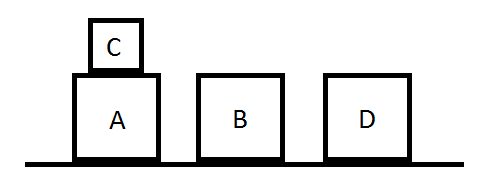
\includegraphics[width=\textwidth]{block-world-3}
  \caption{Block World final state, after Bob's action}
  \label{fig:block-world-3}
\end{figure}

To illustrate the opposite, consider two agents inside a room: the first one, John, seated at its desk and the second one, Mary, standing between John's desk and the door.
After a short conversation regarding a general topic, John, heads toward the door.
Mary, understanding John's intention of getting out of the room, promptly moves aside out of John's way, without John communicating its own intentions.

This action, of Mary stepping aside of John's way, is clearly a social one.
By interpretation of John's action, Mary demonstrated that it has an understanding of John goals and actively acts upon this knowledge.
Mary has an internal representation of John's mind, by other words, Mary is a \textit{mind-reading} agent, the basis of a social agent \cite{castelfranchi:socialactions}.

Mind-reading is the main capability an agent must posses in order to perform social actions.
And as shown in the example, this internal representation of another's agent goals and intentions, needs not be explicitly transmitted, and is, in many cases, interpreted from the agent's behaviour \cite{castelfranchi:socialactions}.

We can now understand that social agents need not only have goals and intentions of their own, but must also be able to understand and model goals and intentions of other agents.

\subsubsection{How do they do it}
\begin{itemize}
\item Comme il Faut
\item Fatima
\item An architecture for believable socially aware agents: MSc Dissertation by Arvand Dorgoly
\item Praxis
\item PsychSim
\end{itemize}
\subsection{Artificial Intelligence in Games}

For games, one of the most important aspects is the player's experience.
The game's flow and immersion are key elements to this experience \cite{ijsselsteijn:userexperience}, and this is where \ac{AI} comes into play.
In the last years, in order to improve plauer's game play experience, the game industry have used \ac{AI} with several different purposes: player experience modelling, procedural content generation, massive-scale game data mining, and \ac{NPC} \ac{AI} \cite{yannakakis:gameairevisited}.

In this section I'm interested in exploring the techniques and tools used for the creation of \ac{NPC}s.
As the name suggests, non playable characters are part of the game but the player cannot control them.
If not the player, then who controls \ac{NPC}s?
The answer is \ac{AI}.
In games, \ac{AI} focus on the creation of characters that behave like humans or animals.

However, game \ac{AI} doesn't always use complex techniques to achieve believable characters, and often, the more complex algorithms produce behaviours that appear stupid \cite{millington:AIgames}.
For example, in Black and White \cite{game:black&white} the player plays the part of a god.
Using a gigantic creature under his control, the player can take over villages, see Fig. \ref{fig:black-and-white}.
\begin{figure}
  \centering
    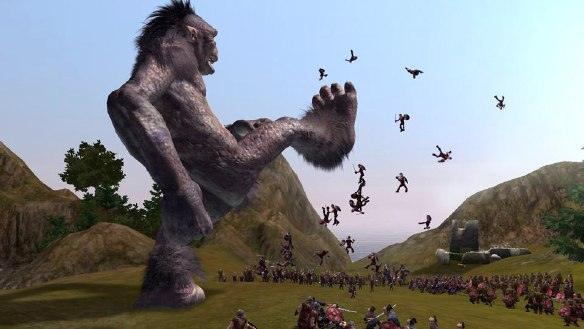
\includegraphics[width=\textwidth]{black-and-white}
  \caption{Black and White, example of using your creature to destroy a village.}
  \label{fig:black-and-white}
\end{figure}
This creature uses reinforcement learning algorithms to learn the behaviours that the player wants him to perform automatically.
But not always the creatures learns want the player wants, learning unwanted behaviours and even failing to learn the most basic ones.

Because of this, and the lack of control on more complex algorithms, game developers sometimes choose to fake it.
"If it looks like a duck, and makes quack, it probably is a duck".
Instead of using complex algorithms, game developers tend to use clever solutions that produce a good behaviour.

In Pacman \cite{game:pacman}, the ghost's behaviour can almost be viewed as each one of them having different personalities.
In Japan, each of them even as a name that characterizes their behaviour almost to the letter: the red ghost, \textit{oikake}, which means "to run down or pursue"; the pink ghost, \textit{machibuse}, meaning "to perform an ambush"; the blue ghost, \textit{kimagure}, meaning "a fickle, moody, or uneven temper"; and the orange ghost, \textit{otoboke}, meaning "pretending ignorance".
By using four different targeting functions (check Fig. \ref{fig:ghosts-targeting})\ref{pacman:dossier}, the game developers have managed to create interesting and challenging opponents that have believable behaviours.

\begin{figure}
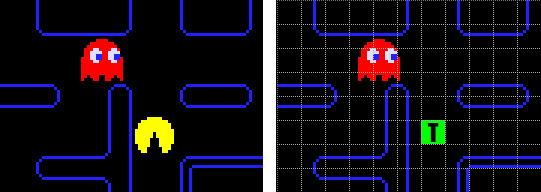
\includegraphics[width=0.5\textwidth]{blinky}
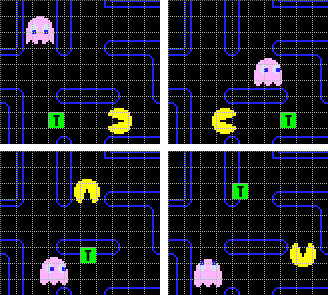
\includegraphics[width=0.5\textwidth]{pinky}
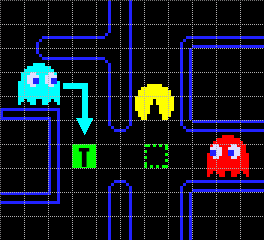
\includegraphics[width=0.5\textwidth]{inky}
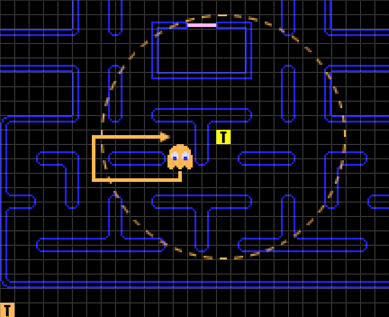
\includegraphics[width=0.5\textwidth]{clyde}
  \caption{Pacman's ghosts targeting functions examples.}
  \label{fig:ghosts-targeting}
\end{figure}

For the remainder of this section I'll follow Millington's work \cite{millington:AIgames} on \ac{AI} for games, exploring three common used techniques: Hacks, Heuristics and Algorithms.
In the end I'll present some common constraints found when building \ac{AI} for games.

\subsubsection{Hacks}
\subsubsection{Heuristics}
\subsubsection{Algorithms}
\subsubsection{Constrains}
